\chapter{テンソルと相対論的ローレンツ力}

今夜はスカラー場から電気力学へと移る。前回の議論で有用なパターンが確立された。すなわち、一つの作用が、場が粒子に及ぼす影響と、粒子が場に及ぼす反作用の両方を記述するのである。最終的にはこのパターンを電磁場に適用するが、その前に、計算の対称性を明らかにするのに十分強力な記法が必要である。

この準備作業は飾りではない。マイナス記号、ゼロ、等号、そしてベクトル記法は、それぞれ、言葉で繰り返さなければならない考えを圧縮している。テンソル記法も相対性理論に対して同じことをする。上下の添字、縮約、変換則が整えば、電気的な力と磁気的な力は自ら一つの四次元方程式にまとまるであろう。

\section{四元ベクトルと添字の経済性}

\subsection{上付き成分と下付き成分}

ギリシャ文字の添字は四次元時空座標のすべてにわたり、ラテン文字の添字は三次元空間座標のみにわたる：
\begin{equation}
\mu,\nu,\rho,\sigma=0,1,2,3,
\qquad
m,n=1,2,3.
\end{equation}
一般的な反変四元ベクトルは\(A^\mu=(A^0,A^1,A^2,A^3)\)である。ここで用いる規約では、
\begin{equation}
\eta_{\mu\nu}
=
\begin{pmatrix}
-1&0&0&0\\
0&1&0&0\\
0&0&1&0\\
0&0&0&1
\end{pmatrix},
\qquad
A_\mu=\eta_{\mu\nu}A^\nu .
\label{eq:sr6-metric-lowering}
\end{equation}
したがって、添字を下げると時間成分の符号が変わり、空間成分はそのままである：
\begin{equation}
A_0=-A^0,
\qquad
A_m=A^m.
\label{eq:sr6-component-lowering}
\end{equation}
平坦な時空では、この操作はこれだけのことであるが、同じ記法は一般相対性理論においてより豊かな幾何学的意味を獲得するであろう。

\begin{figure}[htbp]
\centering
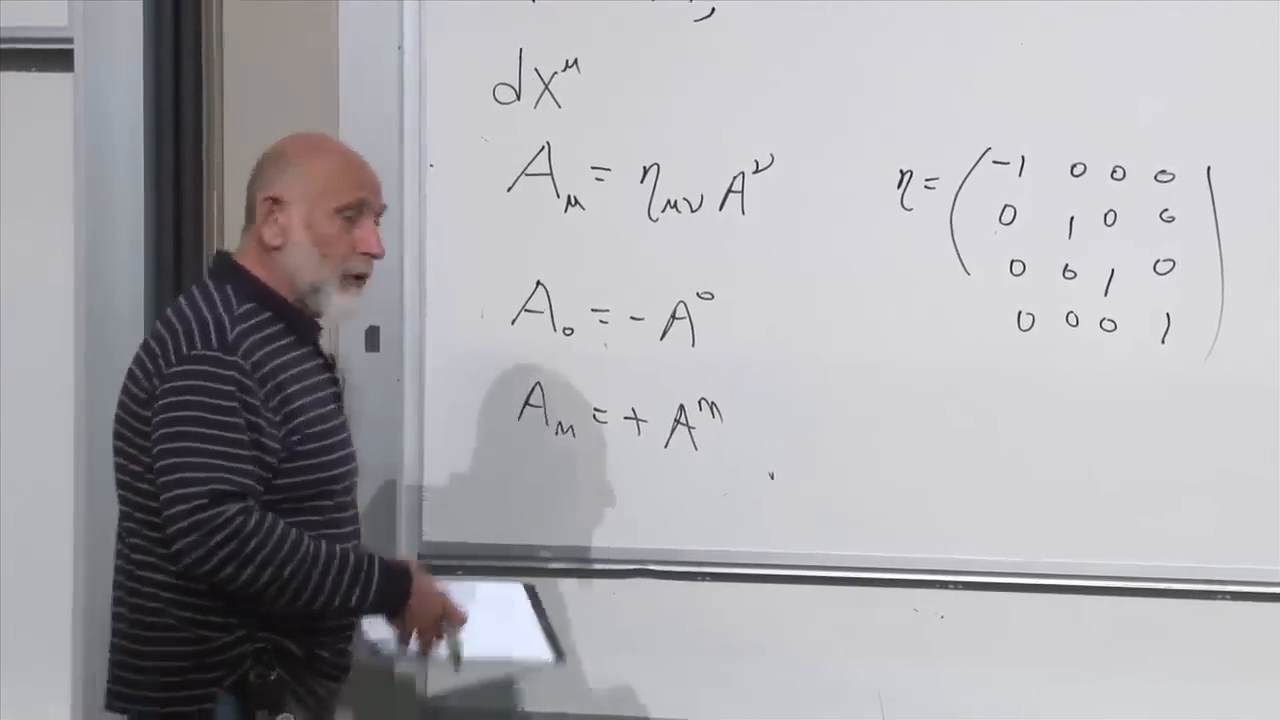
\includegraphics[width=0.90\textwidth]{lecture_06_figure_01.png}
\caption{ミンコフスキー計量と四元ベクトルの添字を下げる成分規則。}
\lectureframe{00:07:45}
\end{figure}

アインシュタインの総和規約は、添字が上に一度、下に一度繰り返されるときに用いられる。したがって、縮約
\begin{equation}
A_\mu B^\mu
=
-A^0B^0+A^1B^1+A^2B^2+A^3B^3
\label{eq:sr6-vector-contraction}
\end{equation}
はスカラーである。和がこの上--下の繰り返しの形をとらない場合には、総和記号を明示的に表示する。

\subsection{微分は下付き添字を伴う}

四つの微分演算子は次のようにまとめられる：
\begin{equation}
\partial_\mu
\equiv
\frac{\partial}{\partial x^\mu}.
\end{equation}
スカラー場\(\phi(x)\)に作用すると、それらは共変ベクトル
\(\partial_\mu\phi\)を形成する。添字の位置を最も手早く理解するには、無限小変位を考えることである：
\begin{equation}
d\phi
=
\frac{\partial\phi}{\partial x^\mu}\,dx^\mu
=
\partial_\mu\phi\,dx^\mu.
\label{eq:sr6-total-differential}
\end{equation}
左辺は隣接する事象におけるスカラー値の差であり、したがってスカラーである。\(dx^\mu\)は反変であるから、それと縮約される対象は共変でなければならない。

\begin{classroomqa}
\audiencequestion{\(x^\mu\)が上付き添字をもつのなら、なぜ\(x^\mu\)に関する微分が下付き添字を生じるのか。}
\lecturerresponse{微分変化\(d\phi=\partial_\mu\phi\,dx^\mu\)がスカラーだからである。反変変位がそのスカラーを生じるには、共変勾配と縮約するしかない。したがって、微分の添字の位置は、分数の見た目だけではなく、その変換則によって定まる。\lecturetimestamp{00:10:10}}
\end{classroomqa}

\begin{figure}[htbp]
\centering
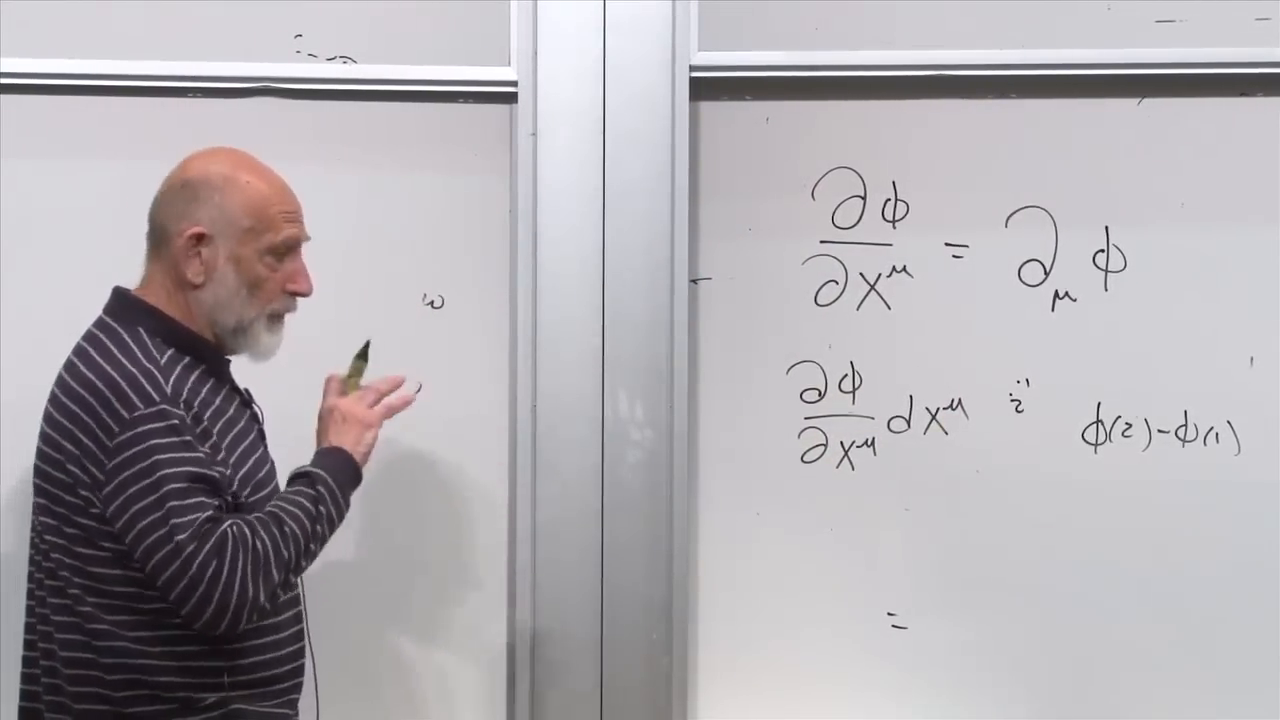
\includegraphics[width=0.90\textwidth]{lecture_06_figure_02.png}
\caption{スカラー微分\(d\phi\)が\(\partial_\mu\phi\)を共変ベクトルとして同定する。}
\lectureframe{00:11:05}
\end{figure}

同じ規則がもう一つのスカラーを与える。\(B^\mu(x)\)が四元ベクトル場ならば、
\begin{equation}
\partial_\mu B^\mu
\label{eq:sr6-four-divergence}
\end{equation}
はその四元発散である。これは時間成分の時間微分と、対応する空間成分の三つの空間微分を組み合わせる。

\begin{figure}[htbp]
\centering
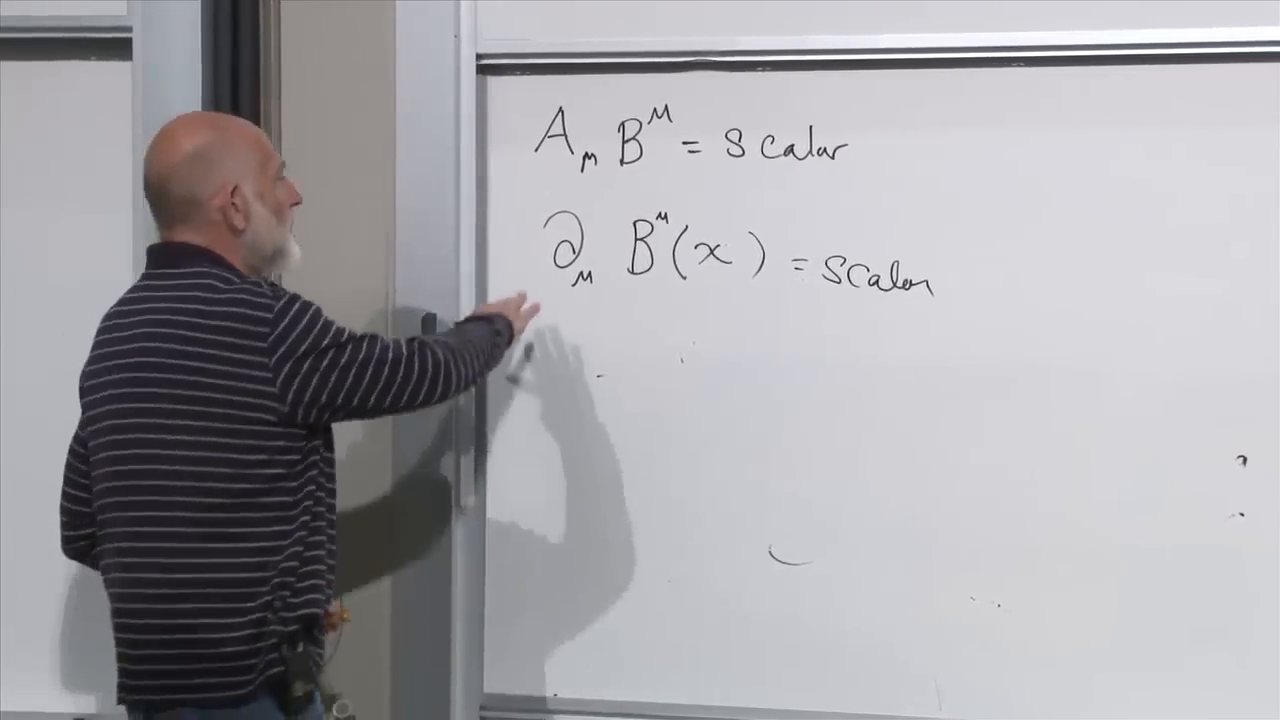
\includegraphics[width=0.90\textwidth]{lecture_06_figure_03.png}
\caption{二つのスカラー縮約：\(A_\mu B^\mu\)と四元発散\(\partial_\mu B^\mu(x)\)。}
\lectureframe{00:14:00}
\end{figure}

これらすべてには三次元の類似物がある。ユークリッド三次元空間では計量が単位行列であるから、ラテン文字の添字を上げても下げても何も変わらない。したがって、都合のよいときには空間添字を上下に動かすが、時空添字の区別は引き続き注意深く保つ。

\section{行列形式のローレンツ変換}

スカラーとベクトルはその変換の仕方によって定義される。スカラーは同じ値を保つが、反変四元ベクトルは
\begin{equation}
(A^\mu)'=L^\mu{}_\nu A^\nu.
\label{eq:sr6-vector-transform}
\end{equation}
に従う。見えている添字\(\mu\)は自由添字であり、両辺に現れる。繰り返される添字\(\nu\)は総和され、最終的な成分方程式からは消える。

ここで\emph{ローレンツ変換}には、空間的回転だけでなくブーストも含まれる。ブーストは任意の軸に沿うことができる。回転はブーストと合成して一般的な変換を生じうる。空間的回転それ自体は時間座標を変えない。

\begin{classroomqa}
\audiencequestion{空間を回転させるとき、時間は完全に影響を受けないままなのか。}
\lecturerresponse{はい。通常の空間的回転では時間成分は変わらない。そのような回転は、時間と空間を混ぜる変換とともに、ローレンツ群に含まれる。\lecturetimestamp{00:16:27}}
\end{classroomqa}

\(x\)軸に沿った速さ\(v\)のブーストについて、\(c=1\)とすると、
\begin{equation}
L^\mu{}_\nu
=
\begin{pmatrix}
\gamma&-\gamma v&0&0\\
-\gamma v&\gamma&0&0\\
0&0&1&0\\
0&0&0&1
\end{pmatrix},
\qquad
\gamma=\frac{1}{\sqrt{1-v^2}}.
\label{eq:sr6-boost-matrix}
\end{equation}
\((t,x,y,z)^{\mathsf T}\)を掛けると
\begin{equation}
\begin{aligned}
t'&=\gamma(t-vx),\\
x'&=\gamma(x-vt),\\
y'&=y,\\
z'&=z.
\end{aligned}
\end{equation}
講義では、行列を黒板で完成させる際にゼロと二つの単位成分が与えられる。

\begin{figure}[htbp]
\centering
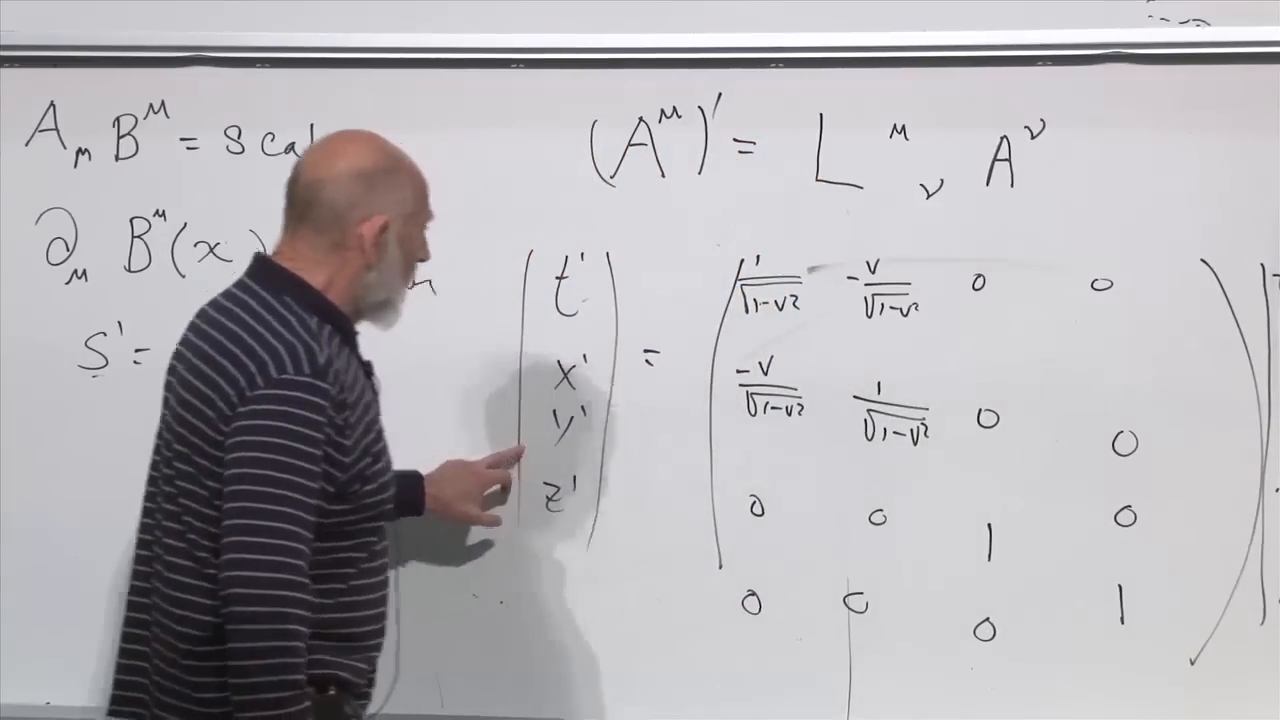
\includegraphics[width=0.90\textwidth]{lecture_06_figure_04.png}
\caption{列\((t,x,y,z)^{\mathsf T}\)に作用する\(x\)方向のブースト行列。}
\lectureframe{00:21:35}
\end{figure}

\(y\)--\(z\)面内の角度\(\theta\)の回転は代わりに
\begin{equation}
R_{yz}(\theta)
=
\begin{pmatrix}
1&0&0&0\\
0&1&0&0\\
0&0&\cos\theta&\sin\theta\\
0&0&-\sin\theta&\cos\theta
\end{pmatrix}.
\label{eq:sr6-yz-rotation}
\end{equation}
となる。これは
\begin{equation}
y'=y\cos\theta+z\sin\theta,
\qquad
z'=-y\sin\theta+z\cos\theta,
\end{equation}
を述べており、一方で\(t\)と\(x\)は固定されたままである。\eqref{eq:sr6-boost-matrix}や\eqref{eq:sr6-yz-rotation}のような行列の積は、より一般的なローレンツ変換を生成する。

\begin{figure}[htbp]
\centering
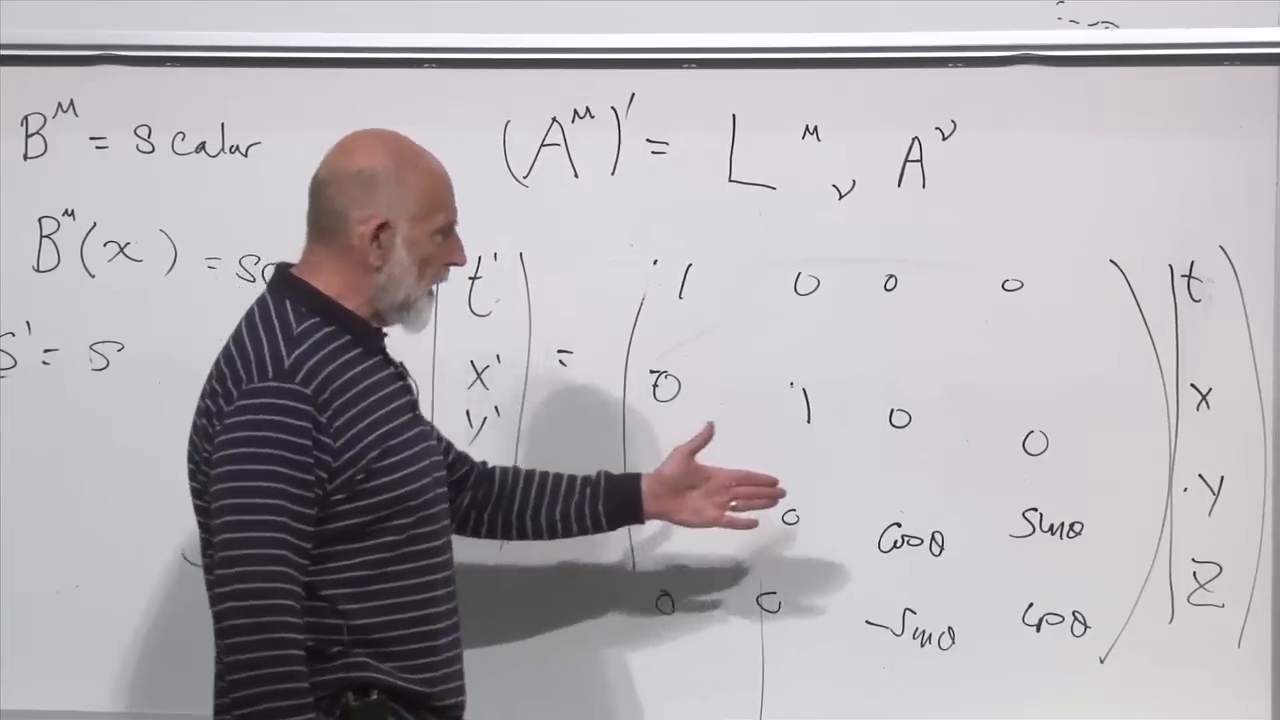
\includegraphics[width=0.90\textwidth]{lecture_06_figure_05.png}
\caption{\(y\)--\(z\)面内の純粋な回転であり、\(t\)と\(x\)は変わらない。}
\lectureframe{00:23:10}
\end{figure}

共変ベクトルは、逆の添字配置をもつ行列によって変換される：
\begin{equation}
(A_\mu)'=M_\mu{}^\nu A_\nu.
\label{eq:sr6-covector-transform}
\end{equation}
黒板での聴衆による訂正が、一時的に繰り返された自由添字を捉えている。左辺の和をとっていない\(\mu\)は、右辺でも和をとっていない添字でなければならない。この二つの行列は同じ物理的な座標系の変更を表しており、
\begin{equation}
M=\eta L\eta,
\qquad
\eta^{-1}=\eta.
\label{eq:sr6-M-L-relation}
\end{equation}
によって関係づけられる。最後の恒等式は、\(\eta\)のすべての対角成分がそれ自身の逆元であることから直ちに従う。

\begin{figure}[htbp]
\centering
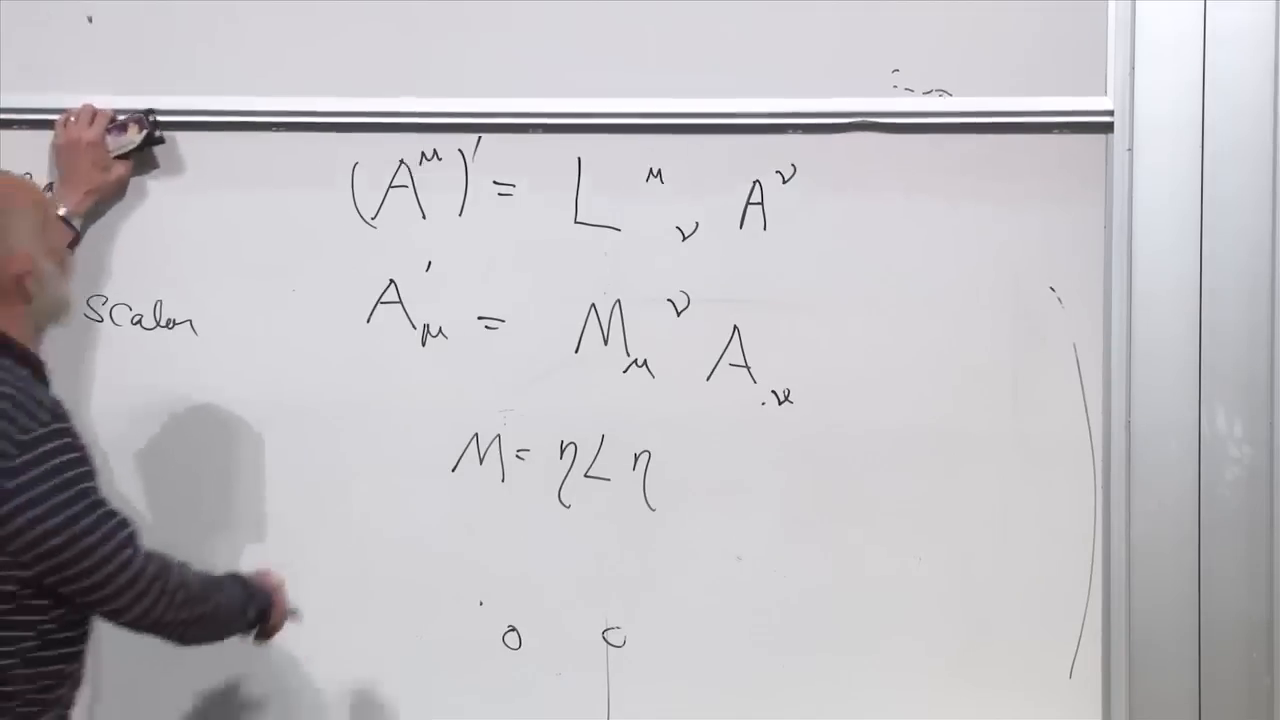
\includegraphics[width=0.90\textwidth]{lecture_06_figure_06.png}
\caption{\(M=\eta L\eta\)によって関係づけられる反変および共変の変換則。}
\lectureframe{00:25:20}
\end{figure}

中心となる考え方がここで得られる：四元ベクトルとは、その成分が時空座標と平行に変換される対象である。

\section{テンソル：各添字に対する一つの変換}

\subsection{ベクトルの積から定義へ}

スカラーは階数ゼロのテンソル、ベクトルは階数一のテンソル、二つの添字をもつ対象は階数二のテンソルである。二つのベクトルから始めて
\begin{equation}
T^{\mu\nu}=A^\mu B^\nu.
\label{eq:sr6-simple-tensor}
\end{equation}
を形成する。\(4\times4=16\)個の成分がある。それらは\(A^0B^0\)および\(A^0B^1\)から\(A^3B^3\)にわたる。記号\(T^{\mu\nu}\)はこの配列全体を表し、一つの数ではない。

各ベクトルを別々に変換すると
\begin{align}
(A^\mu)'&=L^\mu{}_\sigma A^\sigma,\\
(B^\nu)'&=L^\nu{}_\tau B^\tau,
\end{align}
となり、したがって
\begin{equation}
(T^{\mu\nu})'
=
L^\mu{}_\sigma L^\nu{}_\tau T^{\sigma\tau}.
\label{eq:sr6-rank-two-transform}
\end{equation}
となる。各テンソル添字はそれぞれ自身のローレンツ行列を受け取る。ダミー添字\(\sigma\)と\(\tau\)は、各対が整合している限り自由に改名できる。

\begin{classroomqa}
\audiencequestion{この並べ替えは、行列とベクトル成分が可換であることを仮定しているのか？}
\lecturerresponse{これらは通常の古典的数であり、非可換な量子演算子ではないので、可換である。さらに、同じローレンツ行列が両方の添字に作用している。この計算には順序の問題はない。\lecturetimestamp{00:31:56}}
\end{classroomqa}

この規則は直ちに階数三に拡張される：
\begin{equation}
(T^{\mu\nu\lambda})'
=
L^\mu{}_\sigma
L^\nu{}_\tau
L^\lambda{}_\kappa
T^{\sigma\tau\kappa},
\label{eq:sr6-rank-three-transform}
\end{equation}
同様に任意の階数にも拡張される。ベクトルへの特定の因数分解ではなく、この変換則がテンソルの定義である。例えば、
\begin{equation}
A^\mu B^\nu+C^\mu D^\nu
\end{equation}
は一般には二つのベクトルの一つの積として書けないが、それでもテンソルである。

\begin{figure}[htbp]
\centering
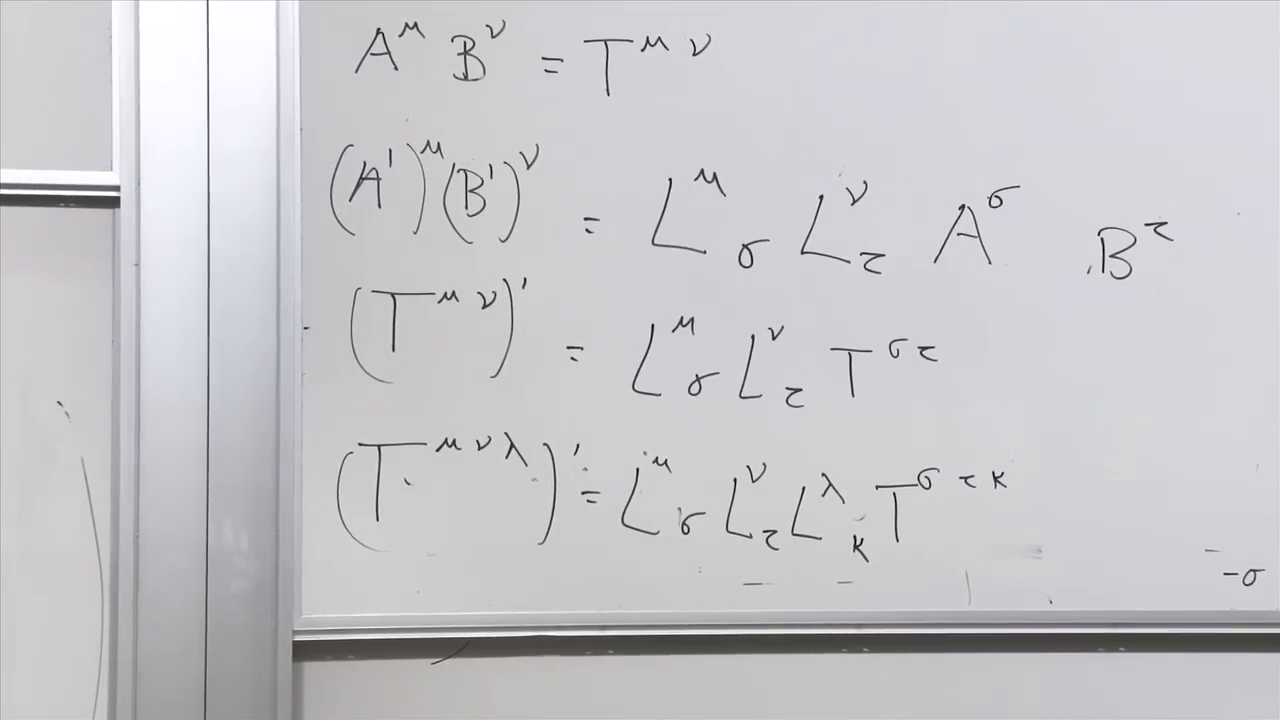
\includegraphics[width=0.90\textwidth]{lecture_06_figure_07.png}
\caption{ベクトルの積から階数二および階数三のテンソル変換則への黒板の階段。}
\lectureframe{00:33:20}
\end{figure}

\begin{classroomqa}
\audiencequestion{階数二のテンソルによる行列の積は、成分ごとに何を意味するのか？}
\lecturerresponse{二つの出力添字を固定し、二つの隠れた添字について和をとる。例えば、
\[
(T^{31})'=L^3{}_\sigma L^1{}_\tau T^{\sigma\tau}.
\]
\(\sigma\)と\(\tau\)はどちらも四つの値をとるので、この一つの出力成分は十六個の項を含む。\lecturetimestamp{00:34:35}}
\end{classroomqa}

\begin{figure}[htbp]
\centering
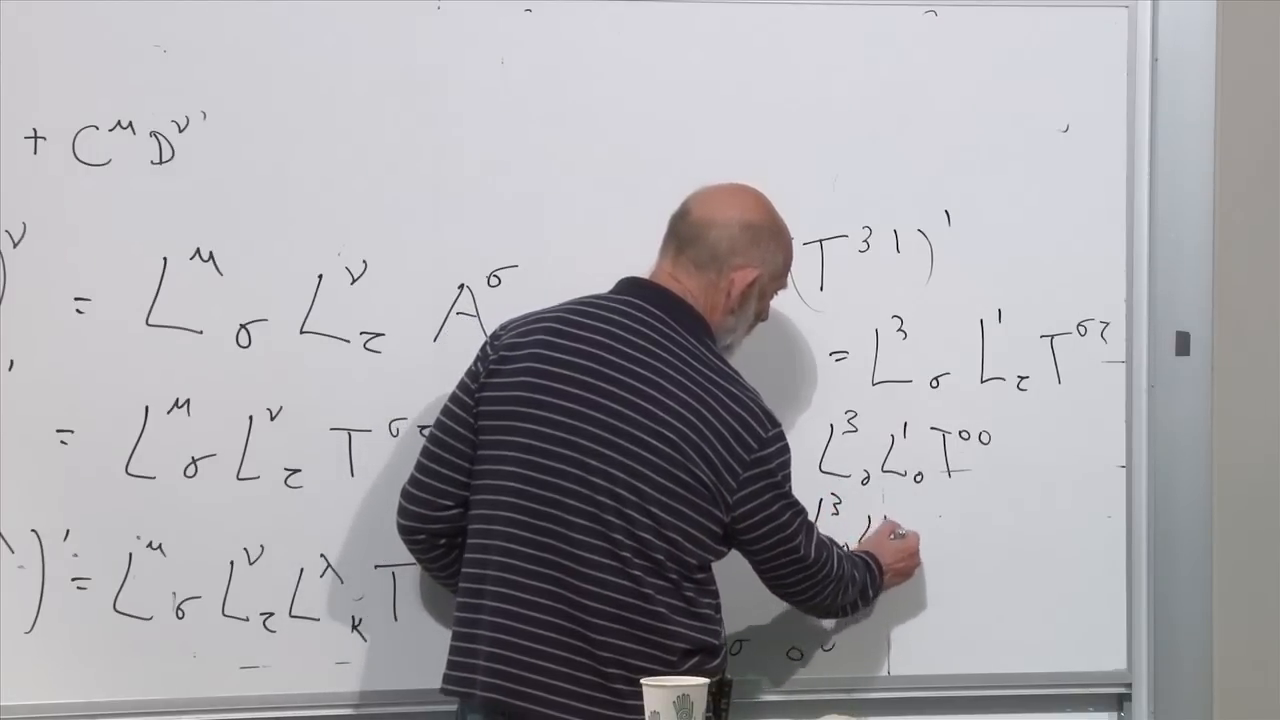
\includegraphics[width=0.90\textwidth]{lecture_06_figure_08.png}
\caption{固定された成分\((T^{31})'\)を展開すると、二つの独立な和が明示される。}
\lectureframe{00:35:55}
\end{figure}

テンソル方程式には決定的な利点がある。二つのテンソルがある座標系で等しい成分をもてば、変換則によりそれらはすべての座標系で等しい。同様に、テンソルのすべての成分がある座標系でゼロならば、テンソル全体がすべての座標系でゼロである。一つの成分がゼロであるだけでは十分でなく、すべての成分がゼロでなければならない。これが、テンソル間で書かれた方程式がその真理性を一つの慣性系から別の慣性系へと運ぶ理由である。

\subsection{テンソル添字の上げ下げ}

テンソルの添字はベクトルの添字とまったく同じように下げられる：
\begin{equation}
T^\mu{}_\nu=T^{\mu\sigma}\eta_{\sigma\nu}.
\label{eq:sr6-tensor-lowering}
\end{equation}
\eqref{eq:sr6-metric-lowering}における対角計量では、下げられた時間添字はそれぞれ一つの負符号に寄与する。したがって、
\begin{equation}
T_{00}=T^{00},
\qquad
T_{01}=-T^{01}.
\label{eq:sr6-tensor-component-signs}
\end{equation}
最初の等式は二つの符号変化を含み、二番目は一つだけを含む。

\begin{figure}[htbp]
\centering
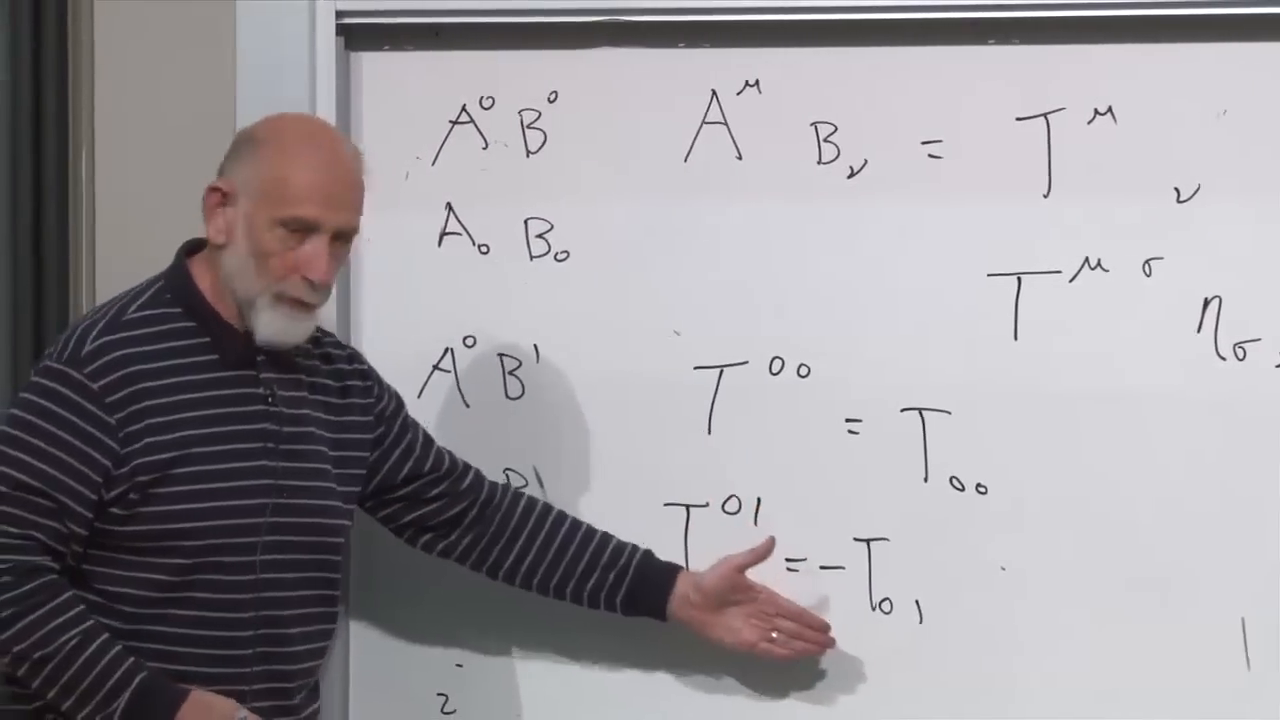
\includegraphics[width=0.90\textwidth]{lecture_06_figure_09.png}
\caption{二つのテンソル添字を下げる例：二つの時間添字は二つの負符号を与え、一つの時間添字は一つを与える。}
\lectureframe{00:41:00}
\end{figure}

\begin{classroomqa}
\audiencequestion{共変形と反変形の両方を保つことはなぜ有用なのか？単なる簡潔な記法以上のものがあるのか？}
\lecturerresponse{現在の計算では、直接の利点は簡潔な縮約とミンコフスキー符号の自動的な管理である。ベクトルとコベクトルの間にはより深い幾何学的な区別があるが、それは一般相対性理論でよりよく展開される。平坦な時空では添字の規則が非常に効率的であるため、通常はそれらを直接扱って計算する。\lecturetimestamp{00:41:26}}
\end{classroomqa}

\begin{classroomqa}
\audiencequestion{テンソルは常に4つの成分をもつのでしょうか、それともそれは相対性理論に特有のものなのでしょうか。}
\lecturerresponse{各添字の範囲は空間の次元によって定まる。4次元時空における1階のテンソルは4つの成分をもち、2階のテンソルは16個の成分をもつ。3次元では対応する数は3と9である。テンソルの規則そのものは次元に依存しない。\lecturetimestamp{00:42:55}}
\end{classroomqa}

\begin{classroomqa}
\audiencequestion{共変な対象と反変な対象はもっと幾何学的に記述できるのでしょうか。}
\lecturerresponse{はい、それらには幾何学的な解釈があるが、今それを追及すると電気力学がさらに後回しになってしまう。この講義では変換規則と添字操作の規則で十分であり、幾何学的な区別は一般相対性理論において避けられなくなる。\lecturetimestamp{00:43:51}}
\end{classroomqa}

\section{対称性、反対称性、電磁テンソル}

一般の2階のテンソルでは、添字を交換すると成分が変わる：
\begin{equation}
T^{\mu\nu}\neq T^{\nu\mu}.
\end{equation}
実際、\(A^\mu B^\nu\) と \(A^\nu B^\mu\) は一般には異なり、特定の成分 \(A^0B^1\) と \(A^1B^0\) は一致する必要はない。

重要な特別な場合が2つある。対称テンソルは
\begin{equation}
T^{\mu\nu}=T^{\nu\mu},
\end{equation}
を満たし、具体的な対称な組み合わせは
\begin{equation}
A^\mu B^\nu+A^\nu B^\mu.
\end{equation}
である。反対称テンソルは
\begin{equation}
F^{\mu\nu}=-F^{\nu\mu},
\label{eq:sr6-antisymmetry}
\end{equation}
を満たし、組み合わせ
\begin{equation}
A^\mu B^\nu-A^\nu B^\mu.
\end{equation}
も同様である。\eqref{eq:sr6-antisymmetry} で添字を等しく置くと
\begin{equation}
F^{00}=-F^{00},
\qquad
F^{00}=0,
\end{equation}
となり、同じ議論によってすべての対角成分が除かれる。したがって \(4\times4\) の反対称テンソルは6つの独立な成分をもつ。

\begin{figure}[htbp]
\centering
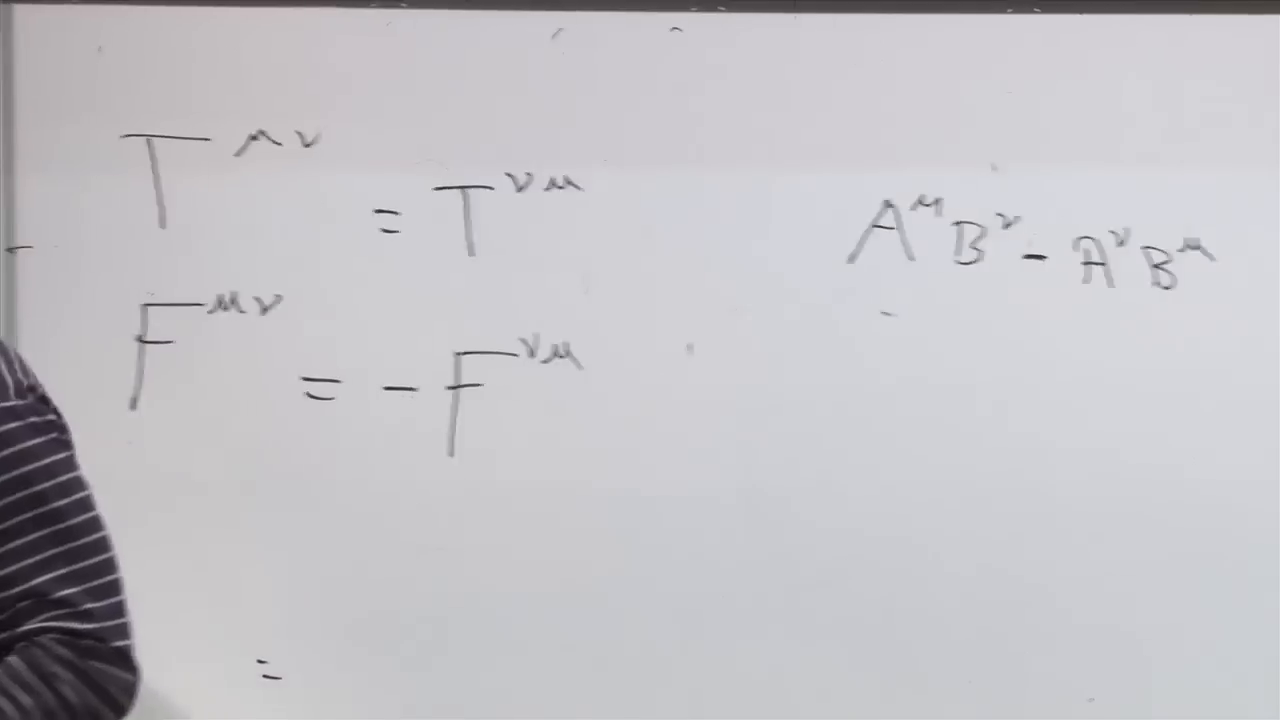
\includegraphics[width=0.90\textwidth]{lecture_06_figure_10.png}
\caption{黒板で比較された対称および反対称の2階テンソル。}
\lectureframe{00:47:20}
\end{figure}

それらの6つの成分は、電場の3つの成分と磁場の3つの成分にとってまさに十分である。黒板に書かれた符号の規約では、
\begin{equation}
F^{\mu\nu}
=
\begin{pmatrix}
0&-E_1&-E_2&-E_3\\
E_1&0&-B_3&B_2\\
E_2&B_3&0&-B_1\\
E_3&-B_2&B_1&0
\end{pmatrix}.
\label{eq:sr6-em-field-tensor}
\end{equation}
対角線を挟んだ反射はすべての符号を反転させる。したがって電場と磁場は独立な相対論的対象ではない。ブーストは空間と時間を混ぜ合わせるのとちょうど同じようにそれらを混ぜ合わせうる：ある慣性系で純粋に電場である場が、別の慣性系では磁場の成分をもちうる。

\begin{figure}[htbp]
\centering
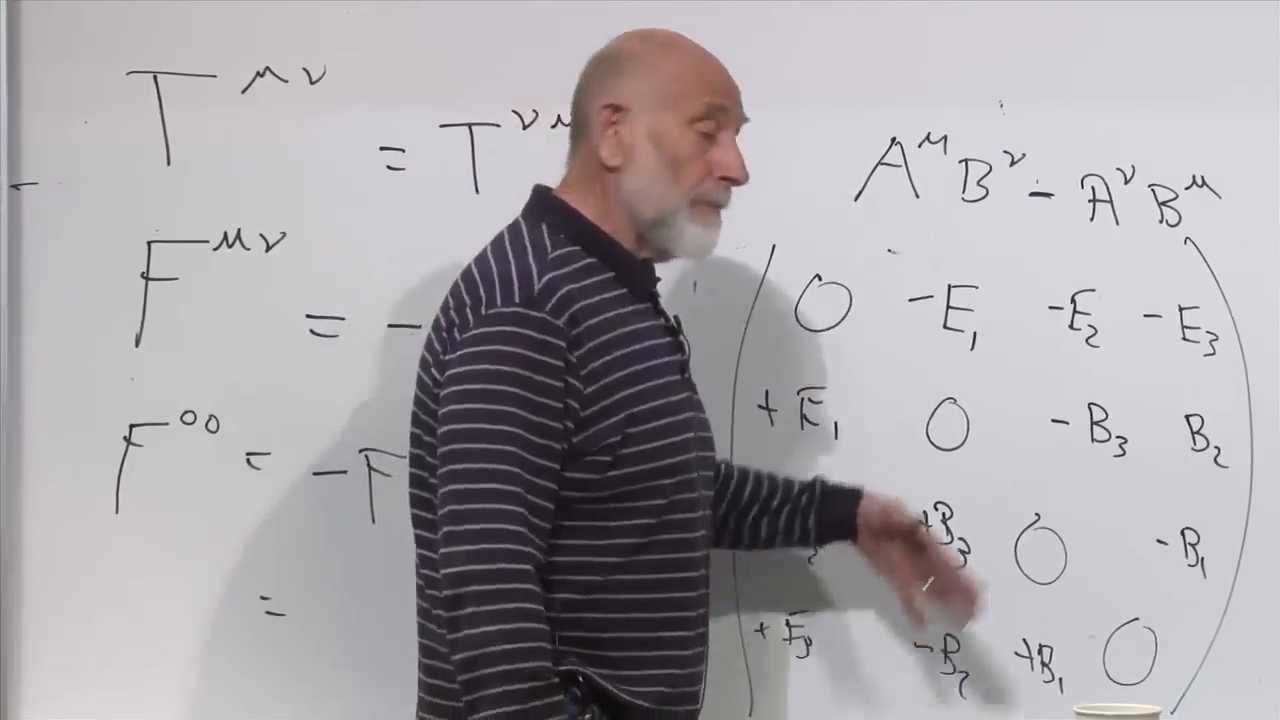
\includegraphics[width=0.90\textwidth]{lecture_06_figure_11.png}
\caption{6つの独立な成分が \(\mathbf E\) と \(\mathbf B\) である完成された反対称配列。}
\lectureframe{00:50:20}
\end{figure}

\eqref{eq:sr6-em-field-tensor} を載せた黒板は、議論が粒子の力学へ移る間も見えたままである。ここで我々は記号 \(A_\mu\) を再び用いるが、それは前の例の一般のベクトルに対してではなく、電磁4元ポテンシャルに対してである。

\section{荷電粒子の作用}

出発点として2つが可能である。場そのものの力学を研究することもでき、それはマクスウェル方程式へ導く。あるいは、与えられた場の中を運動する荷電粒子を研究することもでき、それはローレンツ力を導く。我々は粒子から始める。

低速度では目標は
\begin{equation}
m\mathbf a
=
e\left(\mathbf E+\mathbf v\times\mathbf B\right),
\label{eq:sr6-nonrel-lorentz-force}
\end{equation}
であり、ガウス単位系の版では磁場の項に因子 \(1/c\) が掛かる。我々は \(c=1\) と置く。\eqref{eq:sr6-nonrel-lorentz-force} の2つの項は3次元ベクトル表記では異なって見えるが、相対性理論はそれらが1つの対象の部分であることを明らかにするはずである。

\begin{figure}[htbp]
\centering
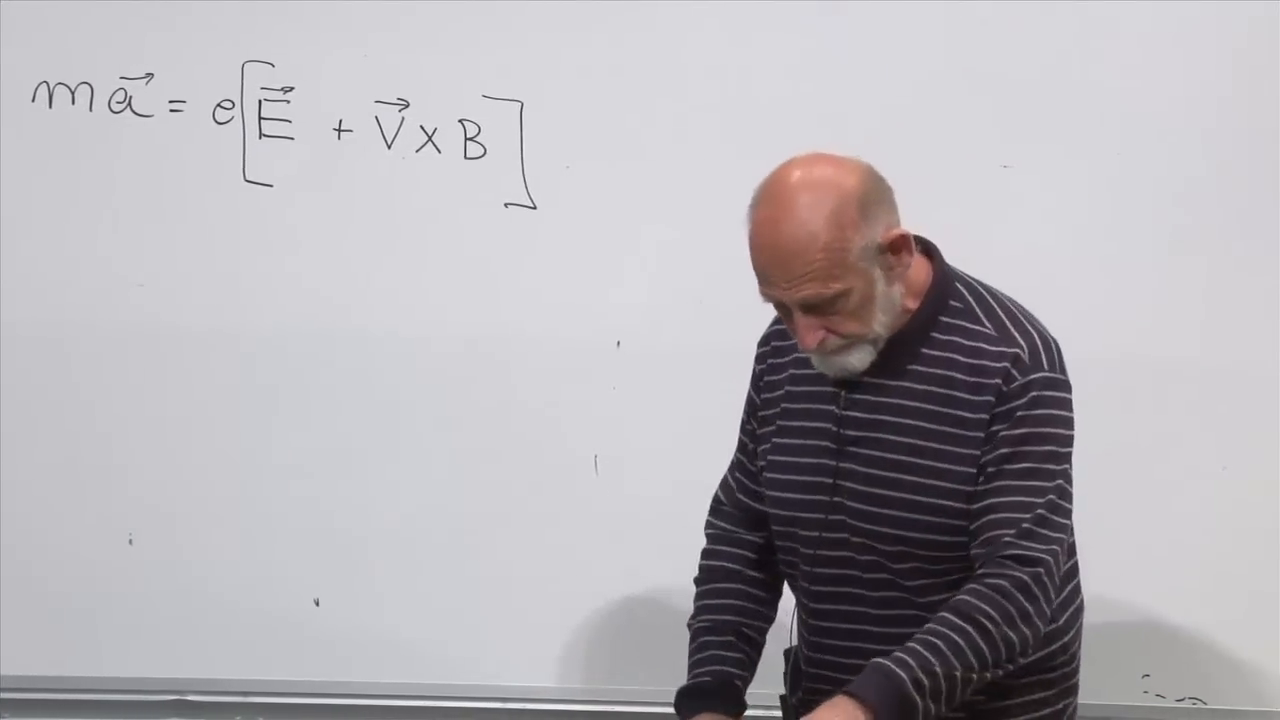
\includegraphics[width=0.90\textwidth]{lecture_06_figure_12.png}
\caption{非相対論的ローレンツ力、すなわち不変な作用が再現しなければならない結果。}
\lectureframe{00:54:00}
\end{figure}

\subsection{自由運動とベクトルポテンシャル}

自由な相対論的粒子に対して、
\begin{equation}
S_{\mathrm{free}}
=
-m\int_1^2 d\tau
=
\int_{t_1}^{t_2}dt\,
\left[-m\sqrt{1-\dot{\mathbf x}^{\,2}}\right],
\label{eq:sr6-free-action}
\end{equation}
ここで
\begin{equation}
\dot{\mathbf x}^{\,2}
=
(\dot x^1)^2+(\dot x^2)^2+(\dot x^3)^2.
\end{equation}
角括弧の中の量は自由粒子のラグランジアンである。その運動量とエネルギーは以前に求められた。我々は作用を保持し、どのような場に依存する項を加えうるかを問う。

\begin{figure}[htbp]
\centering
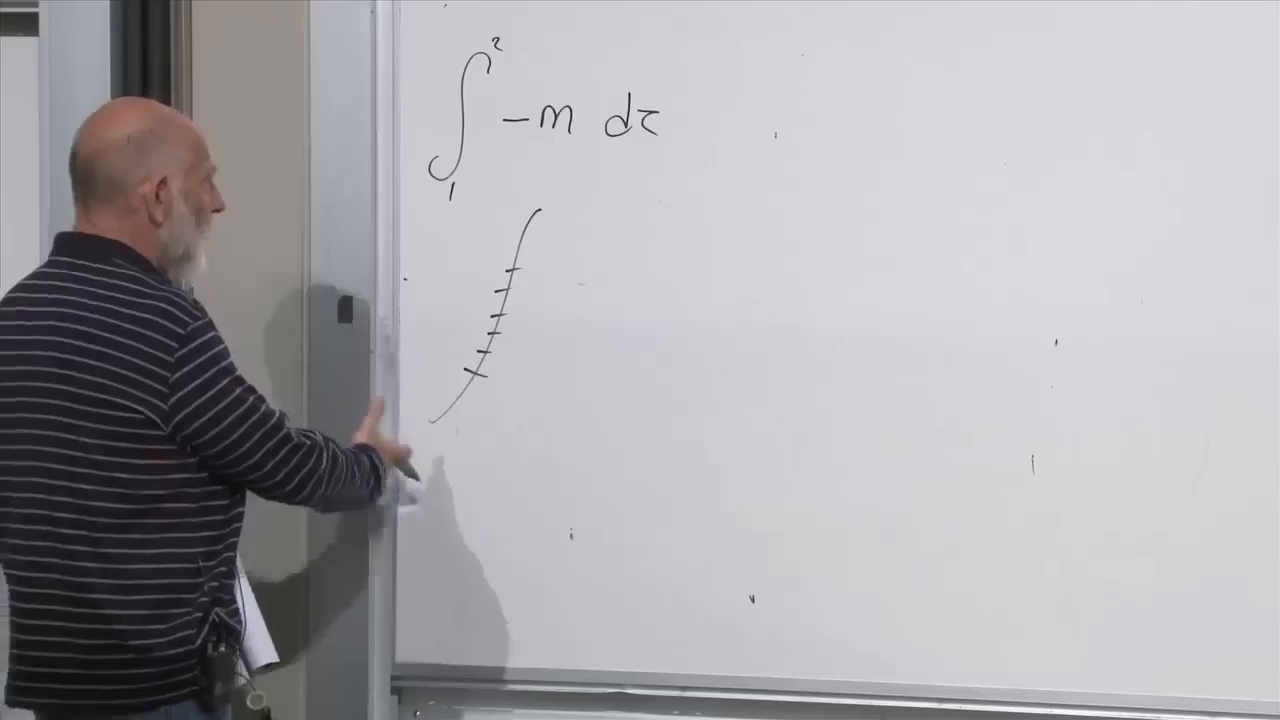
\includegraphics[width=0.90\textwidth]{lecture_06_figure_13.png}
\caption{世界線に沿って蓄積された固有時としての自由作用。}
\lectureframe{00:55:10}
\end{figure}

基本的な電磁変数は4元ベクトルポテンシャル
\(A_\mu(x)\) である。電場と磁場はそれから導かれる。小さな世界線の線分 \(dx^\mu\) に沿って、縮約
\begin{equation}
A_\mu(x)\,dx^\mu
\end{equation}
はスカラーである。それらのスカラーの増分を一方の端点から他方の端点まで加えると、ローレンツ不変な相互作用が得られる：
\begin{equation}
S_{\mathrm{int}}
=
-e\int_1^2 A_\mu(x)\,dx^\mu.
\label{eq:sr6-interaction-action}
\end{equation}
係数 \(e\) は電荷である。全体の符号は歴史的な電荷の規約に属する。規約を変えると \(e\) に割り当てられる符号が変わるだけで、理論の内容は変わらない。

\begin{figure}[htbp]
\centering
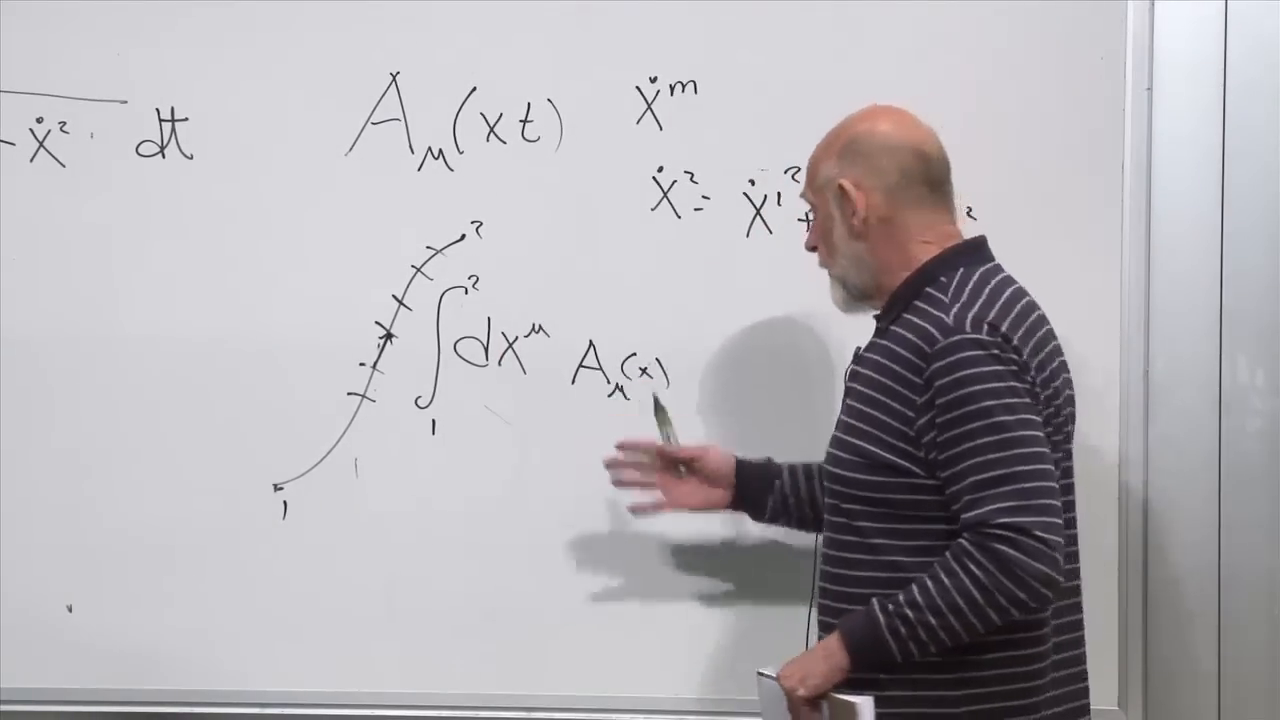
\includegraphics[width=0.90\textwidth]{lecture_06_figure_14.png}
\caption{スカラーの増分 \(A_\mu dx^\mu\) を形成するために4元ポテンシャルと縮約された世界線の線分。}
\lectureframe{00:59:20}
\end{figure}

\subsection{通常時間の形}

よく知られたオイラー--ラグランジュ方程式を用いるために、\eqref{eq:sr6-interaction-action} を \(dt\) で割り、掛ける。
\begin{equation}
\frac{dx^0}{dt}=1,
\qquad
\frac{dx^m}{dt}=\dot x^m,
\end{equation}
であるから、完全な作用は
\begin{equation}
S
=
\int dt\,
\left[
-m\sqrt{1-\dot{\mathbf x}^{\,2}}
-eA_0(x,t)
-e\dot x^m A_m(x,t)
\right].
\label{eq:sr6-complete-particle-action}
\end{equation}
したがって
\begin{equation}
\boxed{
L
=
-m\sqrt{1-\dot{\mathbf x}^{\,2}}
-eA_0
-e\dot x^mA_m
}.
\label{eq:sr6-charged-lagrangian}
\end{equation}
今のところ \(A_\mu(x,t)\) は既知の外部場である。我々は世界線を変分し、場は変分しない。

\begin{figure}[htbp]
\centering
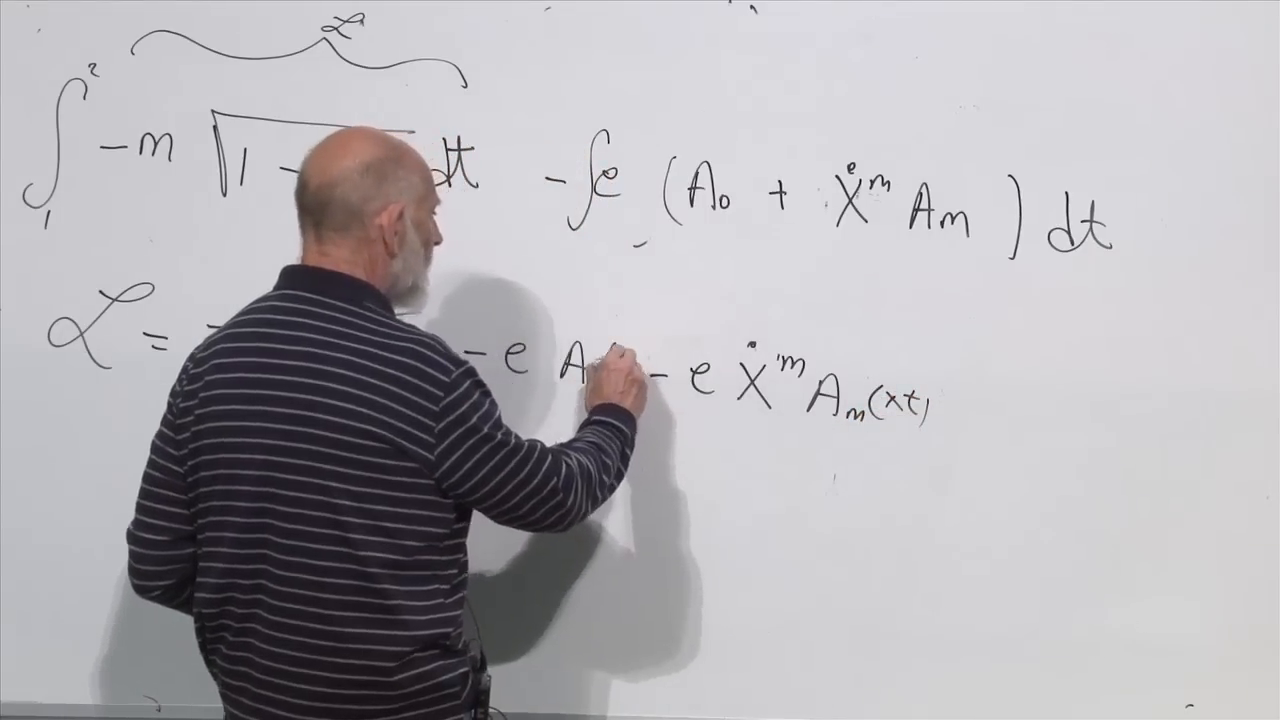
\includegraphics[width=0.90\textwidth]{lecture_06_figure_15.png}
\caption{不変世界線結合を通常時間のラグランジアンとして書き直したもの。}
\lectureframe{01:05:20}
\end{figure}

\section{ローレンツ力の導出}

空間成分\(x^m\)に対して、オイラー--ラグランジュ方程式は
\begin{equation}
\frac{d}{dt}\frac{\partial L}{\partial\dot x^m}
=
\frac{\partial L}{\partial x^m}.
\label{eq:sr6-EL}
\end{equation}
と書ける。速度について微分すると
\begin{equation}
\frac{\partial L}{\partial\dot x^m}
=
\frac{m\dot x_m}{\sqrt{1-\dot{\mathbf x}^{\,2}}}
-eA_m.
\label{eq:sr6-canonical-momentum}
\end{equation}
が得られる。文字\(m\)は残念ながら質量と空間添字の両方の役割を果たす。文脈がそれらを区別する。\eqref{eq:sr6-canonical-momentum}における最初の\(m\)は質量であり、添字\(m\)は3つの空間成分のうちの1つを表す。

\begin{figure}[htbp]
\centering
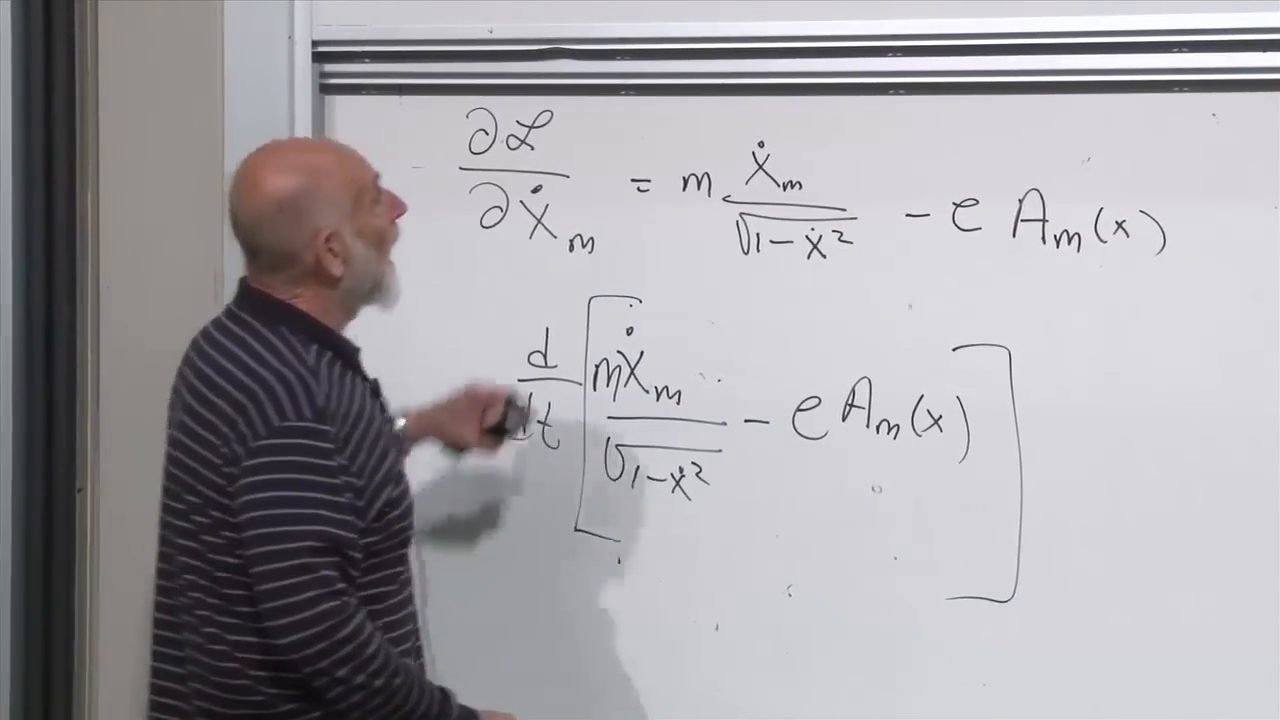
\includegraphics[width=0.90\textwidth]{lecture_06_figure_16.png}
\caption{運動量の微分には、力学的項とベクトルポテンシャル項の両方が含まれる。}
\lectureframe{01:09:20}
\end{figure}

\begin{classroomqa}
\audiencequestion{左辺の最初の試みには項が欠けていないか？}
\lecturerresponse{はい。自由粒子の項だけを微分すると、\(-e\dot x^mA_m\)の速度依存性が落ちてしまう。完全な微分は\(m\dot x_m/\sqrt{1-\dot{\mathbf x}^{\,2}}-eA_m\)である。この補正は不可欠である。その時間微分が電場と磁場の両方の力の一部を与えるからである。\lecturetimestamp{01:08:18}}
\end{classroomqa}

\eqref{eq:sr6-EL}の右辺は
\begin{equation}
\frac{\partial L}{\partial x^m}
=
-e\,\partial_mA_0
-e\,\dot x^n\partial_mA_n.
\label{eq:sr6-position-derivative}
\end{equation}
したがって
\begin{equation}
\frac{d}{dt}
\left(
\frac{m\dot x_m}{\sqrt{1-\dot{\mathbf x}^{\,2}}}
-eA_m
\right)
=
-e\,\partial_mA_0
-e\,\dot x^n\partial_mA_n.
\label{eq:sr6-EL-expanded}
\end{equation}

\begin{classroomqa}
\audiencequestion{この計算で共変空間成分と反変空間成分が入れ替わっていないか？}
\lecturerresponse{上下に動かされてはいるが、ラテン空間添字に対して計量のユークリッド空間ブロックは単位行列である。したがって\(x_m=x^m\)および\(A_m=A^m\)である。符号の変化を生じるのは時間添字だけである。\lecturetimestamp{01:09:29}}
\end{classroomqa}

\begin{classroomqa}
\audiencequestion{繰り返されたラテン添字も和をとるのか？}
\lecturerresponse{はい。繰り返されたラテン添字は\(1\)から\(3\)まで和をとる。繰り返されたギリシャ添字は\(0\)から\(3\)まで和をとる。1つの空間方程式を表す\(m\)のような単独の添字は自由添字であり、和をとらない。質量の記号は添字ではない。\lecturetimestamp{01:10:00}}
\end{classroomqa}

\begin{figure}[htbp]
\centering
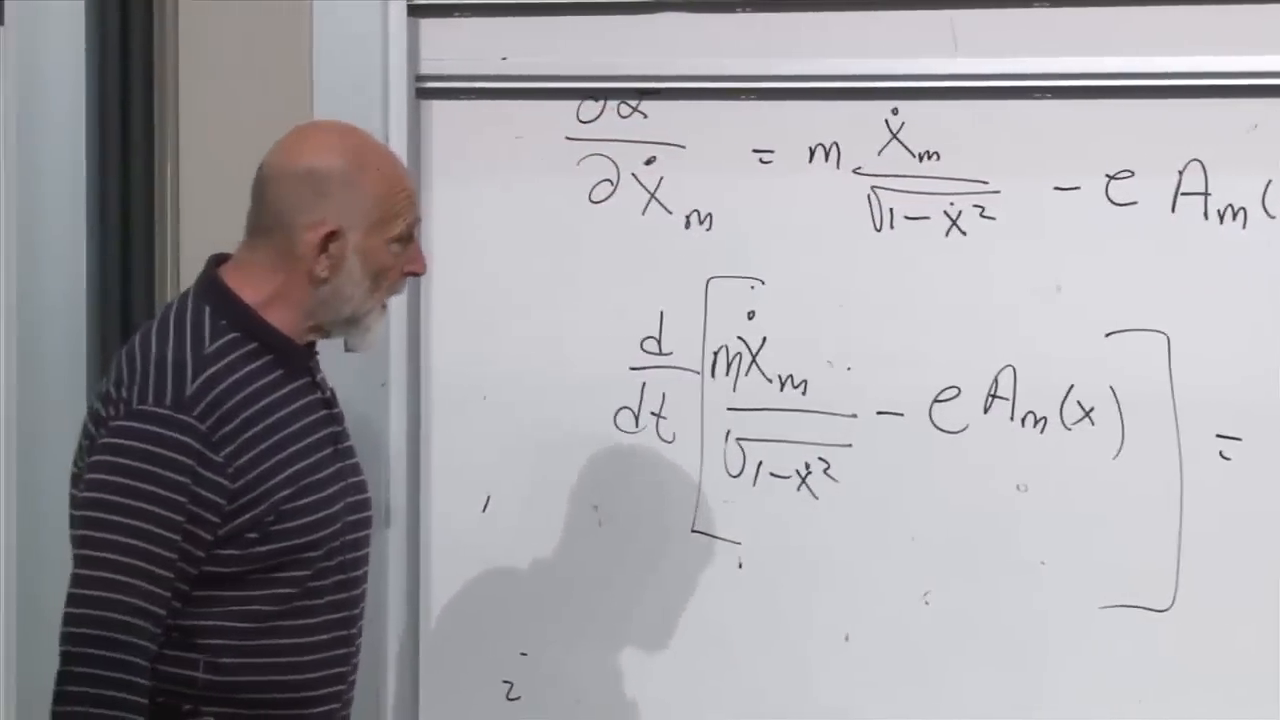
\includegraphics[width=0.90\textwidth]{lecture_06_figure_17.png}
\caption{ベクトルポテンシャルの全時間微分を展開する前のオイラー--ラグランジュ方程式。}
\lectureframe{01:14:20}
\end{figure}

\subsection{運動する世界線に沿った連鎖律}

時間に依存しない場であっても、粒子が異なる位置を通過するため、粒子の経路に沿って変化する。全微分は
\begin{equation}
\frac{dA_m(x(t),t)}{dt}
=
\partial_0A_m+\dot x^n\partial_nA_m.
\label{eq:sr6-convective-derivative}
\end{equation}
である。第1項は陽な時間依存性であり、第2項は\(x^n(t)\)を通じた陰な時間依存性である。

\begin{figure}[htbp]
\centering
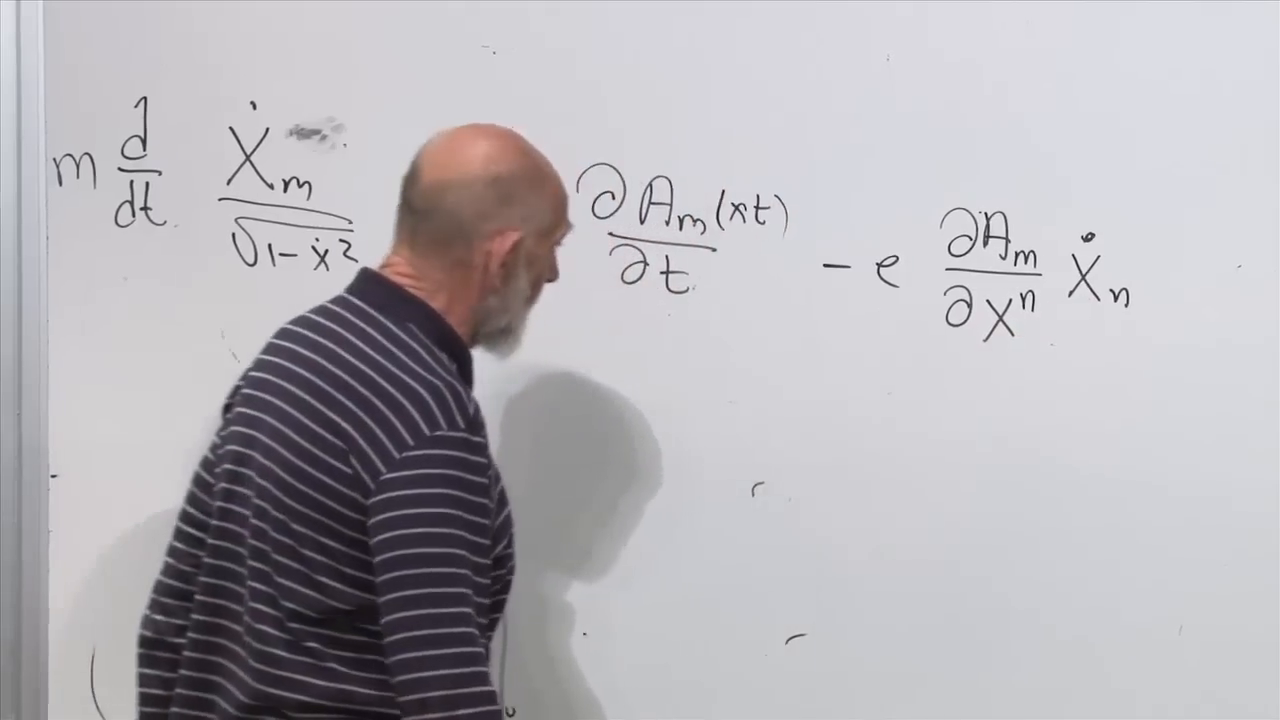
\includegraphics[width=0.90\textwidth]{lecture_06_figure_18.png}
\caption{ベクトルポテンシャルは時間とともに陽に変化し、粒子が空間を運動するにつれて陰にも変化する。}
\lectureframe{01:17:20}
\end{figure}

\eqref{eq:sr6-convective-derivative}を
\eqref{eq:sr6-EL-expanded}に代入し、場の項を右辺に移すと
\begin{equation}
\begin{aligned}
m\frac{d}{dt}
\left(
\frac{\dot x_m}{\sqrt{1-\dot{\mathbf x}^{\,2}}}
\right)
&=
e\left(\partial_0A_m-\partial_mA_0\right)
\\
&\quad +e\dot x^n
\left(\partial_nA_m-\partial_mA_n\right).
\end{aligned}
\label{eq:sr6-grouped-force}
\end{equation}
が得られる。計算はついにその組織原理を見出した。最初の括弧には速度が含まれない。2番目は速度について線形である。これはまさに電気力と磁気力の分割である。

\begin{figure}[htbp]
\centering
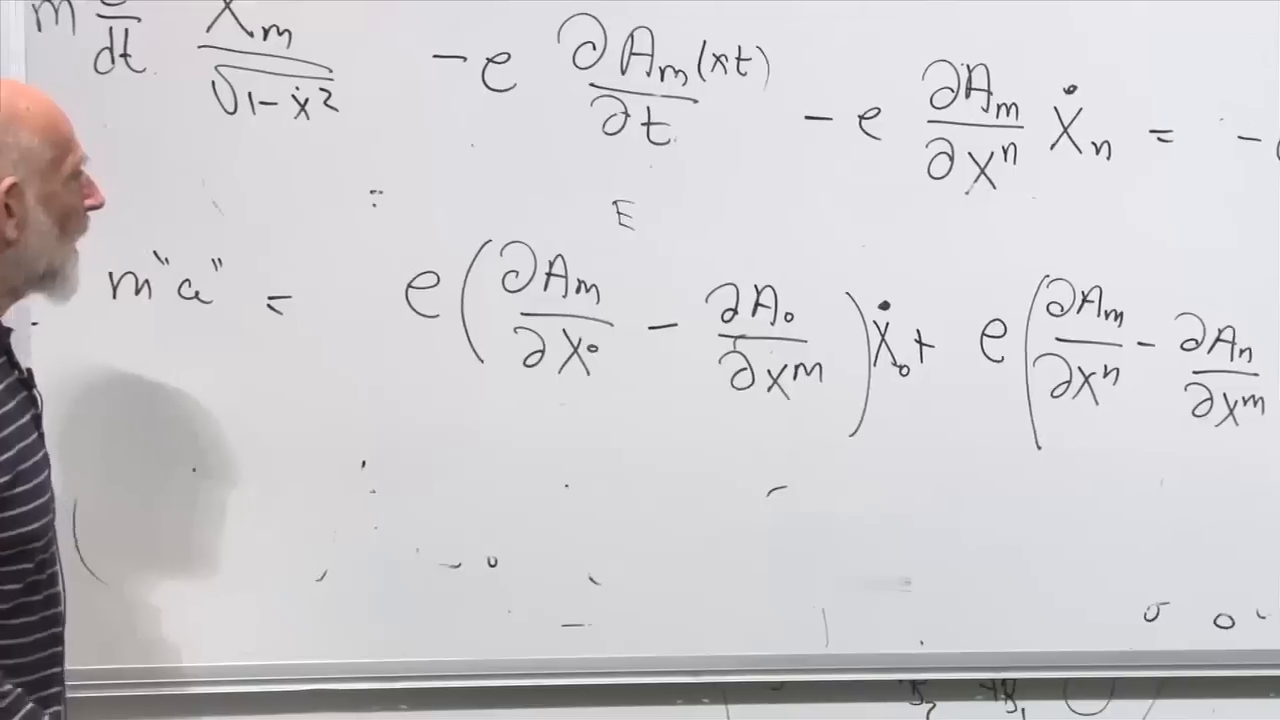
\includegraphics[width=0.90\textwidth]{lecture_06_figure_19.png}
\caption{力の項を、速度に依存しない電気的部分と速度に依存する反対称部分にまとめたもの。}
\lectureframe{01:23:40}
\end{figure}

導出の規約で電気成分を
\begin{equation}
E_m=\partial_0A_m-\partial_mA_0.
\label{eq:sr6-electric-from-potential}
\end{equation}
と定義する。空間的反対称結合
\begin{equation}
C_{mn}
\equiv
\partial_nA_m-\partial_mA_n
\label{eq:sr6-spatial-curl-tensor}
\end{equation}
はベクトルポテンシャルの回転の3つの独立成分を含む。その向きは
\begin{equation}
\dot x^nC_{mn}
=
\left(\mathbf v\times\mathbf B\right)_m.
\end{equation}
となるように選ばれる。したがって式\eqref{eq:sr6-grouped-force}は\eqref{eq:sr6-nonrel-lorentz-force}の相対論的運動量形である。時間微分の下の因子は単位質量あたりの相対論的運動量であり、ニュートン的速度だけではない。

この導出は手で繰り返す価値がある。\eqref{eq:sr6-charged-lagrangian}から始め、\eqref{eq:sr6-EL}の両辺を計算し、連鎖律を適用し、速度依存性に従って項をまとめる。この演習は変分力学、多変数微積分、電気力学の練習を同時に兼ねている。

\begin{classroomqa}
\audiencequestion{なぜ電磁相互作用として\(-e\int A_\mu dx^\mu\)を選ぶのか？}
\lecturerresponse{結合を最終的に決めるのは実験であるが、2つの構造的要請がこれを自然な最初の候補にする。作用は軌道に沿った局所的増分から組み立てられ、各増分はスカラーでなければならない。スカラー\(dx^\mu dx_\mu=d\tau^2\)はすでに自由作用によって表されている。\(dx^\mu\)を場\(A_\mu\)と縮約することは、最も単純な新しい場依存スカラーである。より複雑なスカラーも書くことができ、ゲージ不変性が後に選択を鋭くする。\lecturetimestamp{01:25:34}}
\end{classroomqa}

\begin{classroomqa}
\audiencequestion{マクスウェル方程式も最小作用から導けるか？}
\lecturerresponse{はい。現在の作用は与えられた電磁場中の粒子を支配する。マクスウェル方程式を得るには、場自身の作用を加え、スカラー場の場合とちょうど同じように場自体を変分しなければならない。\lecturetimestamp{01:28:58}}
\end{classroomqa}

\begin{classroomqa}
\audiencequestion{まとめられた力の方程式において、和はどこにあるのか。}
\lecturerresponse{自由な\(m\)は3つの成分方程式のうちの1つに付されたラベルであり、和はとられていない。\(\dot x^n(\partial_nA_m-\partial_mA_n)\)における繰り返された\(n\)は\(1,2,3\)について和がとられている。アインシュタインの記法を用いずに書けば、その項は明示的な\(\sum_{n=1}^{3}\)を伴うであろう。\lecturetimestamp{01:29:26}}
\end{classroomqa}

\begin{classroomqa}
\audiencequestion{なぜ通常の公式をあらかじめ仮定するのではなく、\(\partial_0A_m-\partial_mA_0\)を電場と同定するのか。}
\lecturerresponse{作用は、位置と時間に依存するが粒子の速度には依存しない力の項を生み出した。それはまさに電場の操作的役割である。残りの反対称な項は速度を掛けており、したがって磁場の役割を担う。この計算は、別々の定義をあらかじめ挿入するのではなく、力の法則から場を発見するものと見なすことができる。\lecturetimestamp{01:31:05}}
\end{classroomqa}

\section{明白に共変な力の法則}

\eqref{eq:sr6-grouped-force}の左辺は、まだ明らかに四次元的な形には書かれていない。四元速度
\begin{equation}
u^\mu=\frac{dx^\mu}{d\tau}.
\label{eq:sr6-four-velocity}
\end{equation}
を導入する。その空間成分は
\begin{equation}
u^m
=
\frac{dx^m}{d\tau}
=
\frac{\dot x^m}{\sqrt{1-\dot{\mathbf x}^{\,2}}}.
\end{equation}
を満たす。空間方程式に\(dt/d\tau\)を掛けると、\(d/dt\)が\(d/d\tau\)に変換される：
\begin{equation}
\frac{dt}{d\tau}\frac{d}{dt}
=
\frac{d}{d\tau}.
\end{equation}
したがって左辺は固有加速度の空間部分となる：
\begin{equation}
m\frac{d^2x^m}{d\tau^2}.
\end{equation}

右辺は時間と空間を分離せずに書くことができる：
\begin{equation}
m\frac{d^2x^m}{d\tau^2}
=
e\left(\partial_\nu A_m-\partial_mA_\nu\right)
\frac{dx^\nu}{d\tau}.
\label{eq:sr6-spatial-covariant-force}
\end{equation}
\(\nu=0\)に対しては電場の括弧を再現し、\(\nu=1,2,3\)に対しては磁場の括弧を再現する。

これで両辺は四元ベクトルの変換性をもつ。したがって3つの空間方程式は
\begin{equation}
\boxed{
m\frac{d^2x^\mu}{d\tau^2}
=
e\left(\partial_\nu A^\mu-\partial^\mu A_\nu\right)u^\nu
}.
\label{eq:sr6-covariant-force}
\end{equation}
の成分である。ここで
\begin{equation}
F_{\mu\nu}
\equiv
\partial_\mu A_\nu-\partial_\nu A_\mu,
\label{eq:sr6-F-from-A}
\end{equation}
と定義すれば、この講義で用いた添字の順序と相互作用の符号により、等価な簡潔な形
\begin{equation}
m\frac{du^\mu}{d\tau}
=
-eF^\mu{}_\nu u^\nu.
\label{eq:sr6-covariant-force-F}
\end{equation}
が得られる。
\editorialnote{電磁気学の教科書では、計量の符号、\(A_\mu\)の定義、電荷、および\(F_{\mu\nu}\)の間で符号の配分が異なる。方程式\eqref{eq:sr6-covariant-force}と\eqref{eq:sr6-covariant-force-F}は、作用\(-e\int A_\mu dx^\mu\)から得られた符号と添字の順序を保っている。不変な内容はポテンシャルの反対称化された微分である。}

\begin{figure}[htbp]
\centering
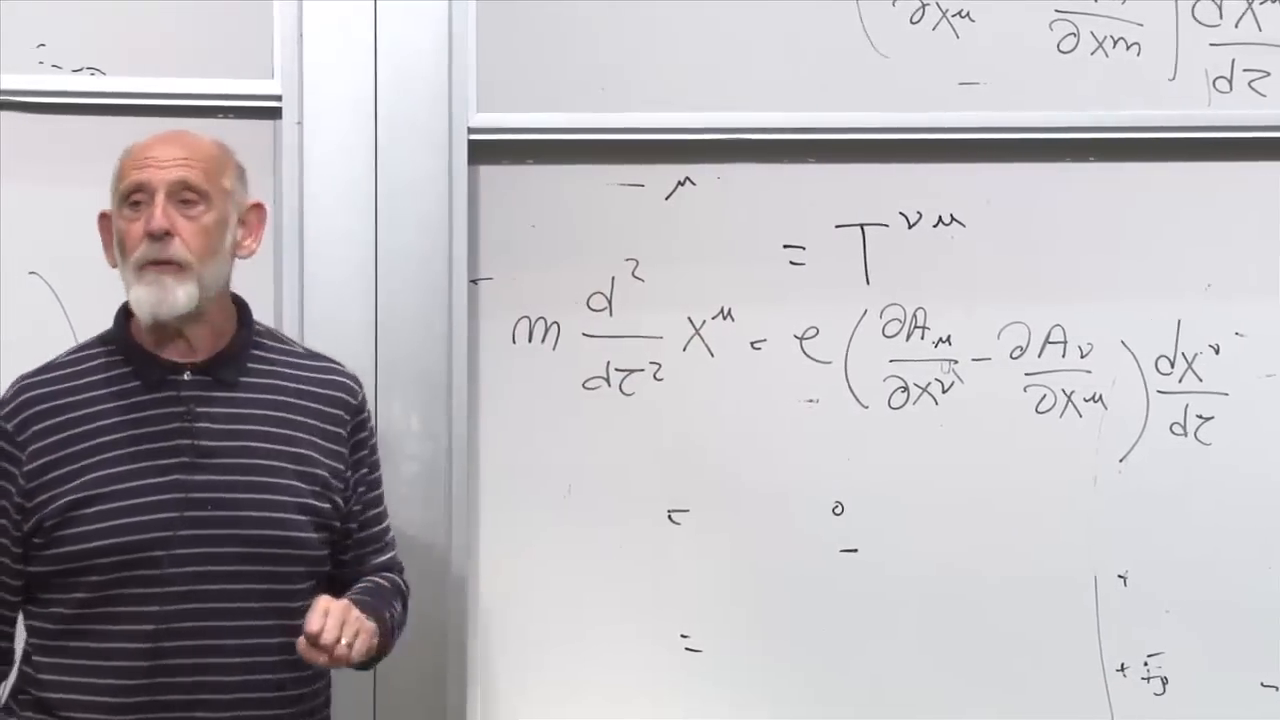
\includegraphics[width=0.90\textwidth]{lecture_06_figure_20.png}
\caption{3つの空間方程式を固有時間を用いて四元ベクトル方程式にまとめたもの。}
\lectureframe{01:42:40}
\end{figure}

\begin{classroomqa}
\audiencequestion{なぜ第4の時間成分の方程式を加えることが正当化されるのか。\(d^2x^0/d\tau^2\)は単にゼロなのか。}
\lecturerresponse{一般にはゼロではない：\(x^0=t\)であるが、\(dt/d\tau=\gamma\)は粒子の速さが変化すると変化する。決定的な論拠は共変性である。スカラー作用はローレンツ不変な方程式を保証する。空間成分が1つの四元ベクトル方程式の成分であると認識されれば、ローレンツ変換はそれらを時間成分と混ぜ合わせる。第4の方程式は他の3つに伴わなければならない。\lecturetimestamp{01:42:40}}
\end{classroomqa}

\subsection{第4成分の意味}

3つの空間成分は相対論的な主張
\begin{equation}
\frac{d\mathbf p}{dt}=\mathbf F.
\end{equation}
である。エネルギーと運動量はそれ自体四元ベクトルの成分であるから、時間成分は対応するエネルギーの収支を記述しなければならない。3次元ベクトルの言葉では、
\begin{equation}
\frac{dK}{dt}=\mathbf F\cdot\mathbf v.
\label{eq:sr6-work-energy}
\end{equation}
である。これは場が粒子に対してする仕事の割合を記録している。磁場の寄与は\(\mathbf v\)に垂直であり仕事をしない。電場の寄与は粒子のエネルギーを変化させる。

\begin{classroomqa}
\audiencequestion{共変性が形式的に第4の方程式を与えるなら、それが物理的意味をもつことをどうやって知るのか。}
\lecturerresponse{最初の3つの成分は、力が運動量を変化させることを述べている。第4の成分は、仕事がエネルギーを変化させることを述べている：\(dK/dt=\mathbf F\cdot\mathbf v\)。エネルギーと運動量は1つの四元ベクトルをなすので、場に対するそれらの応答もまた1つの四成分の主張でなければならない。\lecturetimestamp{01:45:20}}
\end{classroomqa}

\begin{figure}[htbp]
\centering
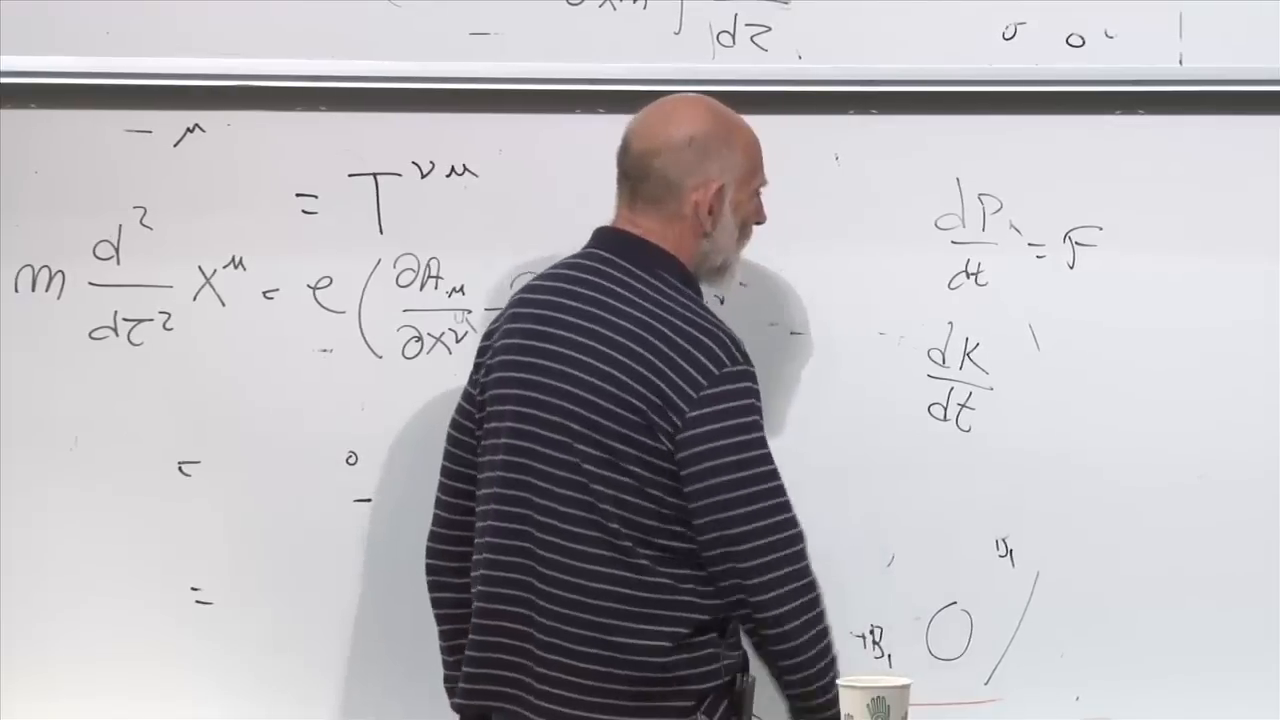
\includegraphics[width=0.90\textwidth]{lecture_06_figure_21.png}
\caption{空間的な法則\(d\mathbf p/dt=\mathbf F\)とその時間成分の相棒である仕事--エネルギーの関係。}
\lectureframe{01:47:10}
\end{figure}

方法は最終的な圧縮よりも重要である。我々は変分をとる前に作用がスカラーであることを要求した。その結果得られた方程式は、事後にその対称性を修復することなく、テンソルへと再編成することができた。現代の場の理論では、これは一般的な設計指針となる：問題の対称性を尊重するようにラグランジアンを構成せよ。

\section{局所性、ローレンツ不変性、そして次の対称性}

相対論的場の理論では3つの原理が繰り返し現れる。2つはすでに用いられた。3つ目は次に展開される。

\subsection{局所性}

局所性とは、粒子や場の変化は時空の中で無限小的に近接して起こることによって支配される、ということを述べている。粒子は自身の世界線上で評価された場に応答し、遠く離れた無関係な値には応答しない。ある点における場は、その点の近傍における場とその導関数に応答し、任意の遠方の値や未来のデータに直接応答するのではない。

したがって場に対しては、作用は局所的な形
\begin{equation}
S
=
\int d^3x\,dt\,
\mathcal L\!\left(\phi,\partial_\mu\phi\right).
\label{eq:sr6-local-action}
\end{equation}
をとる。この積分は各時空点からの寄与を一つずつ加え合わせる。一階導関数は隣接する点との比較を表し、変分原理は微分方程式を生み出す。広く離れた点で場を結合する非局所的な積を想像することもできるが、その方程式ではここでの応答がそこでの条件に直接依存することになる。それは課そうとしている局所的な構造ではない。高階導関数を含む作用も可能であり、興味深い主題をなすが、現在の構成には必要ない。

\begin{figure}[htbp]
\centering
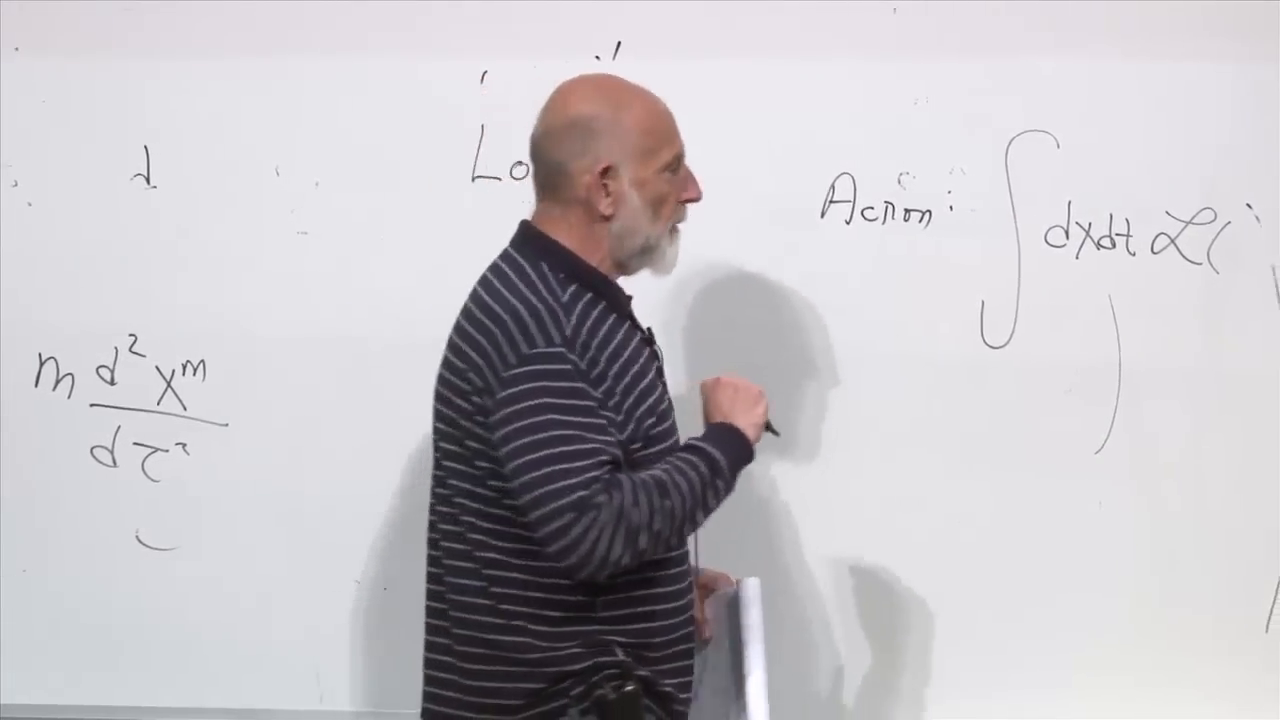
\includegraphics[width=0.90\textwidth]{lecture_06_figure_22.png}
\caption{場とその近傍の導関数から作られた密度の時空積分として表された局所性。}
\lectureframe{01:51:00}
\end{figure}

\begin{classroomqa}
\audiencequestion{\(\partial_\mu\phi\)は四つの導関数成分を表すのか。}
\lecturerresponse{はい。それは\(\phi\)の時間導関数と三つの空間導関数を表し、一つの共変四元ベクトルとしてまとめられている。\lecturetimestamp{01:52:25}}
\end{classroomqa}

\begin{classroomqa}
\audiencequestion{局所性の原理において\emph{近傍}はどのように定量化されるのか。}
\lecturerresponse{導関数によってである。一階導関数はある点における場を無限小的に隣接する点におけるその値と比較する。局所的なラグランジアンは、同じ時空点における場とそのような導関数の有限個の組に依存する。\lecturetimestamp{01:52:55}}
\end{classroomqa}

\begin{classroomqa}
\audiencequestion{局所性の場の版は、たった今完了した粒子の計算にどのように翻訳されるのか。}
\lecturerresponse{粒子のラグランジアンは世界線に沿って局所的である。すなわち、速度を通じて隣接する世界線上の位置に依存し、粒子の現在位置で評価された電磁ポテンシャルに依存する。ここでの粒子の加速度は、遠方の点における場に直接依存しない。\lecturetimestamp{01:53:31}}
\end{classroomqa}

\subsection{ローレンツ不変性}

ローレンツ不変性は、ラグランジアンをスカラーから構成することによって実現される。観測者はそれらのスカラーを異なる時間成分と空間成分に分解することがあるが、作用については一致する。変分によって得られるテンソル方程式は、したがってすべての慣性系で同じ形をとる。

\subsection{ゲージ不変性}

ゲージ不変性が残る原理である。ここではそれが宣言されているが、まだ定義されていない。次の段階で、それは四元ポテンシャルのどの特徴が物理的に意味をもつかを制約し、マクスウェル方程式を生み出す場の作用を導くであろう。

\begin{figure}[htbp]
\centering
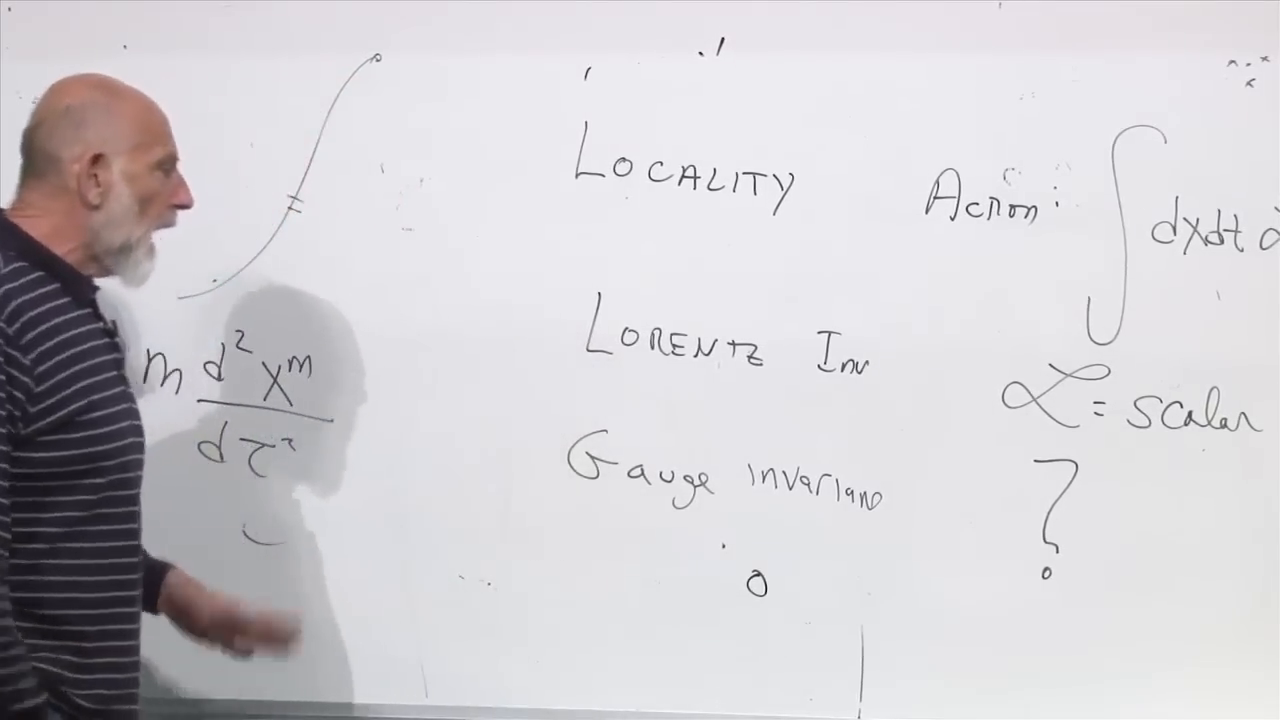
\includegraphics[width=0.90\textwidth]{lecture_06_figure_23.png}
\caption{三つの組織原理：局所性、ローレンツ不変性、ゲージ不変性。}
\lectureframe{01:55:40}
\end{figure}

これらの原理は一般相対性理論、量子電磁力学、Yang--Mills理論、標準模型において繰り返し現れる。粒子種の数などの詳細は理論ごとに異なるが、局所性と対称性がより深い枠組みを与える。したがって実践的な課題は、すべての添字とすべてのまとめられた項を説明できるようになるまでオイラー--ラグランジュ計算をたどり直すことである。ゲージ不変性は、次に同じ電磁作用に対する次の制約として入ってくるであろう。